\documentclass[8pt]{beamer}
% basics
\usepackage{amsfonts}
\usepackage{float}
\usepackage{graphicx}
\usepackage{hyperref} 
\usepackage[labelfont=bf]{caption}
\usepackage{algorithm,algorithmic}
\usepackage{caption}

\newlength\myindent
\setlength\myindent{2em}
\newcommand\bindent{%
  \begingroup
  \setlength{\itemindent}{\myindent}
  \addtolength{\algorithmicindent}{\myindent}
}
\newcommand\eindent{\endgroup}

% unique math expressions:  
\usepackage{amsmath}
\DeclareMathOperator*{\andloop}{\wedge}
\DeclareMathOperator*{\pr}{Pr}
\DeclareMathOperator*{\approach}{\longrightarrow}
\DeclareMathOperator*{\eq}{=}

% \usetheme{Frankfurt}
% \usetheme{Berlin}
\usecolortheme{orchid}
\usetheme{Copenhagen}
% \usefonttheme{serif}
\setbeamertemplate{itemize items}[circle]
\begin{document}
\title{Atomic Consistency Memory in BAMP systems}
\author{Yosef Goren}
\date{}
\frame{
    \titlepage
    On \textbf{'Atomic Read/Write Memory in Signature-Free Byzantine Asynchronous Message-Passing Systems'}.\\
    A paper by:\\
    Achour Mostefaoui, Matoula Petrolia, Michel Raynal, Claude Jard
}

\begin{frame}
    \frametitle{Table of Contents}
    \tableofcontents
\end{frame}

\section{Introduction}
\subsection{Background}
\begin{frame}
    \frametitle{Why care about implementing registers?}
    \begin{block}{What we get}
        This implementation provides a reduction from Message Passing models to Atomic Memory models.
    \end{block}
    \begin{block}{What it can be used for}
        Many distributed algorithms are based on atomic memory; this reduction provides instant implementations
        of these algorithms in message passing systems.
    \end{block}
    \begin{examples}
        \begin{itemize}
            \item - Atomic, multi-writer multi-reader registers 
            \item - Concurrent time-stamp systems
            \item - Atomic snapshot scan
        \end{itemize}
    \end{examples}
\end{frame}

\begin{frame}
    \frametitle{Previous Atomic Register Algorithms}
    %TODO: add ABD, others...
\end{frame}

\subsection{System Model}
\begin{frame}
    \frametitle{\emph{BAMP}: Byzantine Asynchronous Message Passing}
    A distributed system of $n$ processes $p_1, p_2, ... p_n$.
    \begin{block}{Byzantine}
        A byzantine process is one that acts arbitrarily, it may crash or even
        send 'malicious' messages to correct processes.\\
        Let $t$ be the number of byzantine processes, we assume $t<\frac{n}{3}$.
    \end{block}
    \begin{block}{Asynchronous}
        A message sent from $p_i$ to $p_j$ may take any amount of time to arrive.
    \end{block}
\end{frame}

\begin{frame}
    \frametitle{Signature Free}
    Many algorithms cope with byzantine processes by requiring them to sign messages,
    thus requiring assuming cryptographic primitives to be correct, it is not the case here.
\end{frame}

\begin{frame}
    \frametitle{Rliable Broadcast Abstraction}
    Based on a seperate paper, we can use a reliable broadcast algorithm as a 'black box' (in \emph{BAMP} systems).
    \begin{block}{Guarantees}
        A reliable broadcast has the syntax '\emph{r\_brodcast(m)}', and guarantees
        that message the $m$ arrives at all correct processes eventually.
    \end{block}
\end{frame}

\subsection{Solution Requirments}
\begin{frame}
    \frametitle{Atomic Concistency}
    \textbf{Atomic Concistency} is how we intuitively expect memory to be,
    it is also known as Linearizability.
    \begin{block}{A Simple Definition}
        \emph{'for any execution of the system, there is some way of totally ordering
        the reads and writes so that the values returned by the reads are the same
        as if the operations had been performed in that order, with no overlapping.'}\\
    \end{block}
    - 'On Interprocess Communication' (1985), Leslie Lamport.
\end{frame}
\begin{frame}
    \frametitle{Single Writer Multiple Reader Registers (\emph{SWMR})}
    A single process can write; everyone can read.\\
    \begin{block}{Single Writer \& Byzantine Processes}
        If all shared memory can be written by all processes - a single Byzantine process can destroy it.
    \end{block}
    \begin{block}{Local Copies}
    Each process $p_i$ has $Reg_i$, but can only write to \alert{$Reg_i[i]$}.
        \begin{center}
            \begin{tabular}{|c|c|c|}
                \hline
                $p_1$ & $p_2$ & $p_3$ \\
                \hline
                \alert{$Reg_1[1]$} & $Reg_2[1]$ & $Reg_3[1]$ \\  
                $Reg_1[2]$ & \alert{$Reg_2[2]$} & $Reg_3[2]$ \\  
                $Reg_1[3]$ & $Reg_2[3]$ & \alert{$Reg_3[3]$} \\
                \hline
            \end{tabular}\\
        \end{center}
    \end{block}
\end{frame}

\begin{frame}
    \frametitle{ }
\end{frame}

\section{Algorithm}
\subsection{Dealing with Asynchrony}

\begin{frame}[fragile]
    \frametitle{Attempt 1 - No Synchronization}
    \begin{algorithm}[H]
        \begin{algorithmic}[0]
            \STATE \textbf{operation} $REG[i].write(v)$ \textbf{is}
            \bindent
                \STATE $Reg[i].value \leftarrow v$
                \STATE $brodcast$ $WRITE(v)$
            \eindent

            \STATE \textbf{operation} $REG[j].read()$ \textbf{is}
            \bindent
                \STATE $return$ $Reg[j].value$
            \eindent
            
            \STATE \textbf{when a message} $WRITE(v)$ \textbf{arrives} from $p_j$ \textbf{do}
            \bindent
                \STATE $Reg[j].value \leftarrow v$
            \eindent

        \end{algorithmic}
        \caption{Incorrect algorithm with no synchronization}
        \label{alg:seq}
    \end{algorithm}
\end{frame}

\begin{frame}
    \frametitle{Algorithm 1 - Not even eventually consistent}
    \begin{center}
        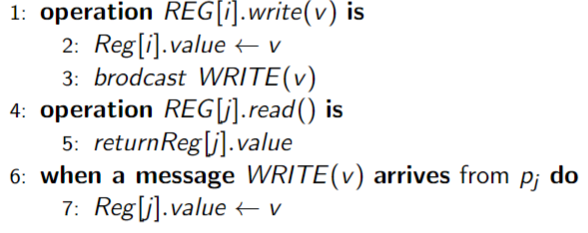
\includegraphics[scale=.7]{resources/alg1_src.png}
        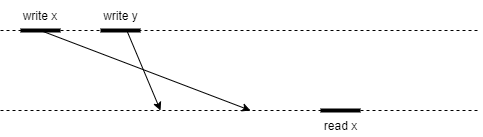
\includegraphics[scale=.5]{resources/alg1_incorrectness.png}
    \end{center}
\end{frame}

\begin{frame}[fragile]
    \frametitle{Attempt 2 - Write Synchronization}
    \begin{algorithm}[H]
        \begin{algorithmic}[0]
            \STATE \textbf{operation} $REG[i].write(v)$ \textbf{is}
            \bindent
                \STATE $sn\leftarrow sn+1$
                \STATE $Reg[i].value \leftarrow v$
                \STATE $brodcast$ $WRITE(v)$
                \STATE $\textbf{wait}$ $got$ $WRITE\_DONE(sn)$ $from$ $all$
            \eindent

            \STATE \textbf{operation} $REG[j].read()$ \textbf{is}
            \bindent
                \STATE $return Reg[j].value$
            \eindent
            
            \STATE \textbf{when a message} $WRITE(v, sn)$ \textbf{arrives} from $p_j$ \textbf{do}
            \bindent
                \STATE $Reg[j].value \leftarrow v$
                \STATE $send$ $WRITE\_DONE(sn)$ $to$ $p_j$
            \eindent

        \end{algorithmic}
        \caption{wait on writes - Sequentially Consistent, but not Linerarizable}
        \label{alg:seq}
    \end{algorithm}
\end{frame}

\begin{frame}
    \frametitle{Algorithm 2 - Not Linearizable due to Read Inversion}
    \begin{center}
        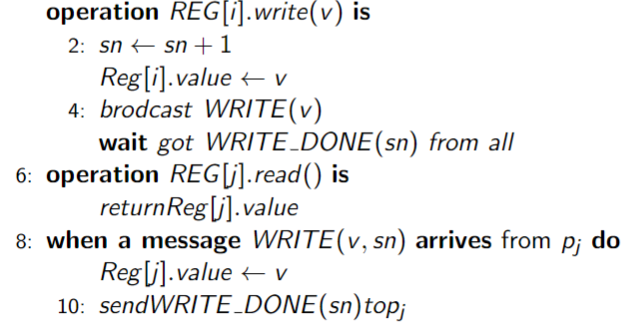
\includegraphics[scale=.63]{resources/alg2_src.png}
        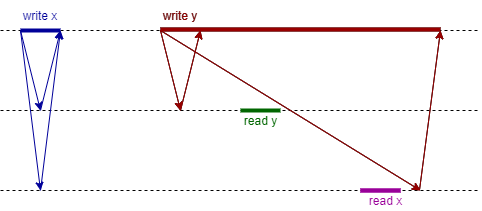
\includegraphics[scale=.5]{resources/alg2_incorrectness.png}
    \end{center}
\end{frame}

\subsection{Dealing with Write Inversion}
\begin{frame}[fragile]
    \frametitle{Attempt 3 - Waiting Read}
    \begin{algorithm}[H]
        \begin{algorithmic}[0]
            \STATE \textbf{operation} $REG[i].write(v)$ \textbf{is}
            \bindent
                \STATE $wsn\leftarrow wsn+1$
                \STATE $Reg[i].value \leftarrow v$
                \STATE $brodcast$ $WRITE(v)$
                \STATE $\textbf{wait}$ $got$ $WRITE\_DONE(wsn)$ $from$ $all$
            \eindent
        \end{algorithmic}
        \caption{Wait on both reads and writes -
            Linearizable but cannot handle faulty processes}
    \end{algorithm}
\end{frame}

\begin{frame}[fragile]
    \frametitle{Attempt 3 - Waiting Read. Cont.}
    \begin{algorithm}[H]
        \begin{algorithmic}[0]
            \STATE \textbf{operation} $REG[j].read()$ \textbf{is}
            \bindent
                \STATE $rsn[j]\leftarrow rsn[j]+1$
                \STATE $brodcast$ $READ(j, rsn[j])$
                \STATE $\textbf{wait}$ $got$ $STATE(wsn_k[j], rsn[j])$ $from$ $each$ $p_k$
                \STATE $sn := max\{rsn_k[j]\mid k\in[n]\}$
                \STATE $\textbf{wait}$ $rsn[j] \geq sn$
                \STATE $when$ $done:$ $w, sn \leftarrow Reg[j]$
                \STATE $brodcast$ $CATCH\_UP(j, sn)$
                \STATE $\textbf{wait}$ $got$ $CATCH\_UP\_DONE(j, sn)$ $from$ $all$
                \STATE $return$ $w$
                % why not just return Reg[j].value when done?
            \eindent
        \end{algorithmic}
        \caption*{}
    \end{algorithm}
\end{frame}

\begin{frame}[fragile]
    \frametitle{Attempt 3 - Waiting Read. Cont.}
    \begin{algorithm}[H]
        \begin{algorithmic}[0]
        \STATE \textbf{when a message} $WRITE(v, sn)$ \textbf{arrives} from $p_j$ \textbf{do}
        \bindent
            \STATE $Reg[j].value \leftarrow v$
            \STATE $send$ $WRITE\_DONE(sn)$ $to$ $p_j$
        \eindent
        \STATE \textbf{when a message} $READ(j, rsn)$ \textbf{arrives} from $p_j$ \textbf{do}
        \bindent
            \STATE $send$ $STATE(Reg[j].sn, rsn)$ $to$ $p_j$
        \eindent
        
        \STATE \textbf{when a message} $CATCH\_UP(j, sn)$ \textbf{arrives} from $p_j$ \textbf{do}
        \bindent
            \STATE $\textbf{wait}$ $Reg[j].sn \geq sn$
            \STATE $send$ $CATCH\_UP\_DONE(sn, rsn)$ $to$ $p_j$
        \eindent
    \end{algorithmic}
        \caption*{}
    \end{algorithm}
\end{frame}

\begin{frame}
    \frametitle{Algorithm 3 - No Read Inversion}
    \begin{center}
        \begin{figure}
            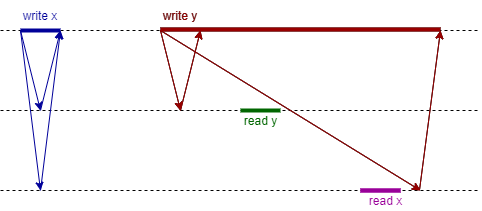
\includegraphics[scale=.35]{resources/alg2_incorrectness.png}
            \caption*{No Read Wait (alg. 2).}
        \end{figure}
        \begin{figure}
            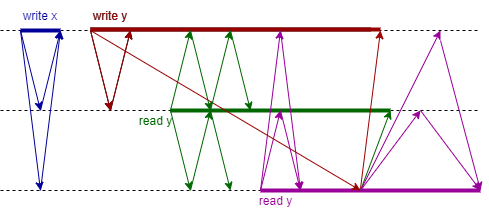
\includegraphics[scale=.35]{resources/alg3_no_read_inversion.png}
            \caption*{With Read Wait (alg. 3).}
        \end{figure}
    \end{center}
\end{frame}

\begin{frame}
    \frametitle{Algorithm 3 - Cannot handle faulty processes}
    \begin{center}
        \begin{alertblock}{Faulty Processes?}
            \begin{itemize}
                \item $p_i$ writes, and waits for $WRITE\_DONE$ from $p_j$.
                \item $p_j$ fails.
                \item $p_i$ is stuck.
            \end{itemize}
        \end{alertblock}
    \end{center}
\end{frame}

\subsection{BAMP Algorithm}

\begin{frame}
    \frametitle{Algorithm 4 - BAMP}
    \begin{block}{Main Idea}
        Use the messages from \textbf{alg. 3} to provide linearizability,
        and use \textbf{majority} and \textbf{reliable brodcast}
        to handle faulty (including byzantine) processes.
    \end{block}
\end{frame}

\begin{frame}
    \frametitle{Initialization and Invocations}
    \begin{center}
        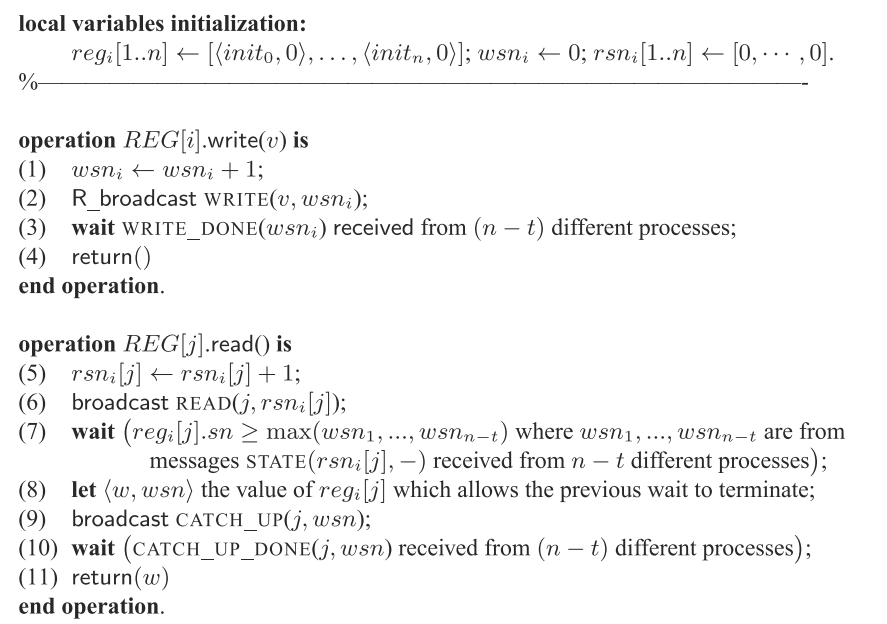
\includegraphics[scale=.7]{resources/alg4_src1.png}
    \end{center}
\end{frame}
\begin{frame}
    \frametitle{Message Handling}
    \begin{center}
        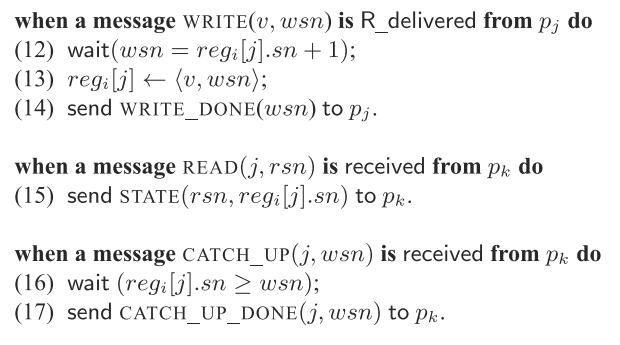
\includegraphics[scale=.7]{resources/alg4_src2.png}
    \end{center}
\end{frame}

\section{Analysis}
\begin{frame}
    \frametitle{Lemma 1}
    \begin{lemma}
        If a correct process $p_i$ recives a message $m$ from a $r\_brodcast(m)$ by another correct process - 
        any other correct process will recive $m$.\\
    \end{lemma}

    \begin{proof}
        Immidiate from the guarantees of the broadcast algorithm.
    \end{proof}

\end{frame}
\begin{frame}
    \frametitle{Lemma 2}
    \begin{lemma}
        Any two sets of processes of size $(n-t)$ mast have
        at least one correct process in common.
    \end{lemma}
\end{frame}
\begin{frame}
    \frametitle{Lemma 2 - Proof}
    \begin{proof}
        Denote the set of processes with $P$, and the set of faulty ones $F$.\\
        Let $Q_1,Q_2\subseteq P$ s.t. $|Q_1|=|Q_2|=n-t$.\\
        \[
            |\overline{Q}_1\cup\overline{Q}_2|\leq |\overline{Q}_1|+|\overline{Q}_2|
            \Rightarrow n-|\overline{Q}_1\cup\overline{Q}_2|\geq n-|\overline{Q}_1|-|\overline{Q}_2|
        \]\[
            \Rightarrow |\overline{\overline{Q}_1\cup\overline{Q}_2}|\geq n-t-t
        \]\[
            \Rightarrow |Q_1\cap Q_2|\geq n-2t>3t-2t=t=|F|
        \]\[
            \Rightarrow \exists p\in Q_1\cap Q_2\notin F
        \]
    \end{proof}
\end{frame}

\subsection{Termination Properties}
\begin{frame}
    \frametitle{Lemma 3}
    \begin{lemma}
        Let $p_i$ be a correct process. Any invocation of $Reg[i].write()$ terminates.
    \end{lemma}
    \begin{proof}
        When $p_i$ invokes $Reg[i].write()$ it sends $WRITE$ to all others,
        due to reliable brodcast - $n-t$ correct processes recive and handle this message
        eventually, thus send back $WRITE\_DONE$.\\
        At some point these arrive and $Reg[i].write()$ temrminates.
    \end{proof}
\end{frame}
\begin{frame}
    \frametitle{Lemma 4}
    \begin{lemma}
    \end{lemma}
\end{frame}

\subsection{Atomicity Properties}
\begin{frame}
    \frametitle{Lemma 5}
\end{frame}
\begin{frame}
    \frametitle{Lemma 6}
    \begin{lemma}
        Let $p_i, p_j$ be two correct processes.\\
        If $read[i,j,x]$ terminates before $write[j,y]$ starts, then $x<y$.
    \end{lemma}
\end{frame}
\begin{frame}
    \frametitle{Lemma 7}
    \begin{lemma}
        Let $p_i, p_j$ be two correct processes.\\
        If $write[i,x]$ terminates before $read[j,i,y]$ starts, then $x\leq y$.
    \end{lemma}
\end{frame}
\begin{frame}
    \frametitle{Lemma 8}
    \begin{lemma}
        Let $p_i, p_j$ be two correct processes.\\
        If $read[i,k,x]$ terminates before $read[j,k,y]$ starts, then $x\leq y$.
    \end{lemma}
\end{frame}

\subsection{Piecing it all together}
\begin{frame}
    \begin{theorem}
        The algorithm showcased implements and array of $n$ SWMR
        registers with atomic concistency, in $BAMP$ with $t<\frac{n}{3}$ systems.
    \end{theorem}
    \begin{proof}
        We have seen required termination properties in lemmas 3,4 and atomicity
        properties in lemmas 5,6,7,8.\\
    \end{proof}
\end{frame}


\section{Conclusions}
\subsection{What we have seen}
\begin{frame}
    \frametitle{What we have seen}
    \begin{block}{Taxonomy and building blocks}
        \emph{Atomic Consistency, SWMR, Reliable Brodcast}
    \end{block}
    \begin{block}{Shared Memory Algorithms}
        We have see some naive ideas for sharing memory, and a correct algorithm for \emph{BAMP} systems.
    \end{block}
    \begin{block}{Correctness Proof}
        Each of the algorithm's wanted properies has been shown.
    \end{block}
\end{frame}

\subsection{Further Work}
\begin{frame}
    \frametitle{Sequential Consistency too much?}
    \begin{alertblock}{Runtime Limitations}
        Requiring a system to implement Atomic Consistency is a very strong requirement
        and often comes at a steep runtime cost.
    \end{alertblock}
    \begin{block}{Alternative Models: $AC\subseteq SC\subseteq RC$}
        Is an algorithm for (only) Sequential Consistency possible?\\
        Or better yet - an algorithm for Release Consistency with some sort of
        \emph{'fence'} operation?
    \end{block}
\end{frame}

\begin{frame}
    \frametitle{Exploding Serial Numbers}
    Number of messages sent is unbounded, memory complexity
    is logarithmic with number of messages sent (due to counters).
    \begin{block}{Reset Serial Numbers}
        Is it possible to add a mechanism to reset the serial numbers?
    \end{block}
    \begin{block}{Mallicious Serial Numbers}
        Is it possible for byzantine processes to cause the serial numbers (within correct processes) to explode?\\
        If so, is it possible to prevent this?
    \end{block}
\end{frame}

\subsection{The End}
\begin{frame}
    \begin{center}
        \textbf{Thanks for listening!}
    \end{center}
\end{frame}

\end{document}